\documentclass[11pt,letterpaper]{article}
\usepackage[lmargin=1in,rmargin=1in,bmargin=1in,tmargin=1in]{geometry}
\usepackage{checkins}


% -------------------
% Content
% -------------------
\begin{document}
\thispagestyle{title}

% 08/22
\checkin{08/22} \textit{True/False}: If $A= (1, 8]$ and $B= (8, 11)$, then $A \cap B= \{ 8 \}$. \pspace

\sol The statement is \textit{false}. The set $A$ is the set of numbers greater than 1 but at most 8, i.e. the numbers less than 8---including 8. Whereas $B$ is the set of numbers greater than 8 but less than 11. The set $A \cap B$ is the set of elements in \textit{both} $A$ and $B$. The only real number that \textit{could} be in both $A$ and $B$ is $8$. However, 8 is in $B$ but not in $A$. Therefore, $8 \notin A \cap B$. But then $A \cap B$ is empty, i.e. $A \cap B= \varnothing$. We can see this by sketching the intervals and seeing that there is no `overlap.' 
	\[
	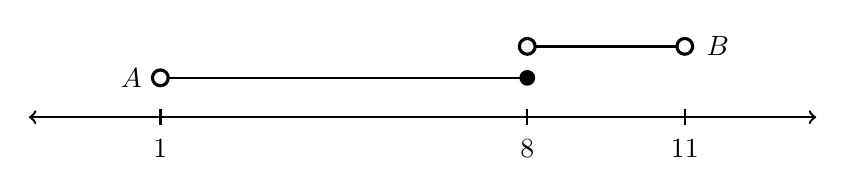
\begin{tikzpicture}
	\draw[line width=0.03cm,<->] (-5,0) -- (5,0);		% Number Line
	
	\draw[line width=0.03cm] (-3.33,-0.1) -- (-3.33,0.1);	% 1 mark
	\draw[line width=0.03cm] (1.33,-0.1) -- (1.33,0.1); 	% 8 mark
	\draw[line width=0.03cm] (3.33,-0.1) -- (3.33,0.1);	% 11 mark
	% A
	\draw[line width=0.03cm] (-3.33, 0.5) -- (1.33,0.5);			% Line
	\draw[fill=white,line width=0.04cm] (-3.33,0.5) circle (0.1);		% Left Label
	\draw[draw=none,fill=black] (1.33,0.5) circle (0.1);			% Right Label
	\node at (-3.7,0.5) {$A$};								% A label
	% B
	\draw[line width=0.03cm] (1.33, 0.9) -- (3.33,0.9);			% Line
	\draw[fill=white,line width=0.04cm] (1.33,0.9) circle (0.1);		% Left Label
	\draw[fill=white,line width=0.04cm] (3.33,0.9) circle (0.1);		% Right Label
	\node at (3.75,0.9) {$B$};								% B label
	% Labels	
	\node at (-3.33,-0.4) {$1$};	% 1 label
	\node at (1.33,-0.4) {$8$};		% 8 label
	\node at (3.33,-0.4) {$11$};	% 11 label
	\end{tikzpicture}
	\] \pvspace{1.3cm}



% 08/26
\checkin{08/26} \textit{True/False}: $\left( \dfrac{y^{-2}}{x^4 x^2} \right)^{-3}= \dfrac{x^{24}}{y^5}$ \pspace

\sol The statement is \textit{false}. Recall that $x^a x^b= x^{a + b}$, $(x^a)^b= x^{ab}$, and $x^{-1}= \frac{1}{x}$. Then we have\dots
	\[
	\left( \dfrac{y^{-2}}{x^4 x^2} \right)^{-3}= \left( \dfrac{y^{-2}}{x^6} \right)^{-3}= \dfrac{y^6}{x^{-18}}= x^{18} y^6
	\] \pvspace{1.3cm}



% 08/27
\checkin{08/27} \textit{True/False}: It is possible to have a right triangle with sides of length $4, 7, 12$. \pspace

\sol The statement is \textit{false}. We know a triangle with sides $a, b, c$ is a right triangle if and only if $a^2 + b^2= c^2$. We have\dots
	\[
	\begin{gathered}
	a^2 + b^2\stackrel{?}{=} c^2 \\
	4^2 + 7^2\stackrel{?}{=} 12^2 \\
	16 + 49\stackrel{?}{=} 144 \\
	65 \neq 144
	\end{gathered}
	\]
Therefore, there exists no such right triangle. In fact, there does not even exist a triangle with such sides. A triangle with sides $a, b, c$ exists if and only if the length of any pairs of sides of the triangle add up to greater than the third. [This is called the triangle inequality.] But $4 + 7= 11 \not> 12$. Therefore, there does not exist a triangle with sides 4, 7, and 12. \pvspace{1.3cm}



% 08/28
\checkin{08/28} \textit{True/False}: Let $f(x)$ be a relation with $f(2)= 7$ and $f(-3)= 7$. Because $f(2)$ and $f(-3)$ are both $7$, $f$ cannot be a function. \pspace

\sol The statement is \textit{false}. A relation is a function if there is only one possible output for a given input, i.e. given an input, one knows with certainty what the output is. We know that $f(2)= 7$ and $f(-3)= 7$; that is, given the inputs of $x= 2$ or $x= -3$, we know the output. The fact that the outputs are the same is irrelevant. There are many functions with the property that $f(2)= 7$ and $f(-3)= 7$. For instance, there must be a linear function through these two points, i.e. $y= 7$. An example of a quadratic function through these points is $y= \frac{7x(x + 1)}{6}$. \pvspace{1.3cm}



% 08/29
\checkin{08/29} \textit{True/False}: Let $f(x)$ be a function. The $y$-intercept of $f(x)$ is $f(0)$ and the $x$-intercept(s) of $f(x)$ are the $x$-values where $f(x)= 0$. \pspace

\sol The statement is \textit{true}. The $y$-intercept is where the graph of the function intersects the $y$-axis, which is the line $x= 0$. But then the $y$-intercept must be the function value at $x= 0$, i.e. $f(0)$. An $x$-intercept is where the graph of the function intersects the $x$-axis, which is the line $y= 0$. But this means the output of the function is zero. Therefore, an $x$-intercept is an $x$-value such that $f(x)= 0$. \pvspace{1.3cm}



% 09/03
\checkin{09/03} If you are walking straight towards a building at a constant speed, then your distance from the building is given by a linear function. The $y$-intercept would represent your initial distance from the building and the slope would represent your walking speed. Furthermore, the $x$-intercept would represent the time you arrive at the building. \pspace

\sol The statement is \textit{true}. Let $D(t)$ denote your distance from the building. Because you are walking towards the building at a constant speed, the distance between you and the building is decreasing at a constant rate. But functions with a constant rate of change are linear. Therefore, $D(t)$ must be linear. We know that the $y$-intercept occurs when $t= 0$, i.e. the $y$-intercept is $D(0)$. But $D(0)$ is the distance you are at $t= 0$, i.e. the start. Therefore, $D(0)$ must denote your initial distance from the building. The slope of $D(t)$ represents the rate of change of your distance from the building. But this distance is only changing because you are walking towards the building. Therefore, the (absolute value of) the slope of $D(t)$ is your walking speed. Finally, an $x$-intercept is an input such that $D(t)= 0$. But $D(t)= 0$ implies that at the given time, your distance from the building is zero, i.e. you have arrived at the building. Therefore, the $x$-intercept of $D(t)$ represents the time you arrive at the building. \pvspace{1.3cm}



% 09/04
\checkin{09/04} Because multiplication is commutative, $(f \circ g)(x)= (g \circ f)(x)$. \pspace

\sol The statement is \textit{false}. While \textit{multiplication} is commutative, $f \circ g$ \textit{does not} represent multiplication. Recall that $f \circ g$ represents function composition, i.e. $(f \circ g)(x)= f \big( g(x) \big)$. Function composition is \textit{not} commutative. For instance, suppose that $f(x)= 5$ and $g(x)= -6$. Then for any $x$, $(f \circ g)(x)= f \big( g(x) \big)= f(-6)= 5$ and $(g \circ f)(x)= g \big( f(x) \big)= g(5)= -6$. But then $(f \circ g)(x) \neq (g \circ f)(x)$ for any $x$. 



\newpage



% 09/05
\checkin{09/05} If $f(x)$ is a function, then $\dfrac{f(-5 + h) - f(-5)}{h}$ represents the average rate of change for $f(x)$ on the interval containing $-5$ and $-5 + h$. If $f(x)$ is linear, this is the slope of $f(x)$. \pspace

\sol The statement is \textit{true}. Recall the average rate of change for a function $f(x)$ on the interval $[a, b]$ is\dots
	\[
	\text{Avg. ROC}_{[a,b]}\, f(x)= \dfrac{f(b) - f(a)}{b - a}= \dfrac{f(a) - f(b)}{a - b}
	\]
That is, the average rate of change for a function on the interval $[a, b]$ is the slope of the line segment through $\big(a, f(a) \big)$ and $\big(b, f(b) \big)$. Because we want the interval containing $-5$ and $-5 + h$, i.e. $[-5, -5 + h]$ or $[-5 + h, -5]$ (depending on whether $h > 0$ or not), the average rate of change on this interval is\dots
	\[
	\dfrac{f(-5 + h) - f(-5)}{(-5 + h) - (-5)}= \dfrac{f(-5 + h) - f(-5)}{-5 + h + 5}= \dfrac{f(-5 + h) - f(-5)}{h}
	\] \pvspace{1cm}



% 09/11
\checkin{09/11} The function $f(x)= 6 - (x + 2)^2$ is quadratic. Furthermore, it is convex and has vertex $(2, 6)$. \pspace

\sol The statement is \textit{false}. Observe that $f(x)= 6 - (x + 2)^2= 6 - (x^2 + 4x + 4)= 6 - x^2 - 4x - 4= -x^2 - 4x + 2$. Therefore, $f(x)$ is quadratic with $a= -1$, $b= -4$, and $c= 2$. We can also see that $f(x)= 6 - (x + 2)^2= -(x + 2)^2 + 6$ is in vertex form---meaning $f(x)$ must be quadratic. Because $a= -1 < 0$, we know that $f(x)$ is concave---not convex. We know that if $a > 0$, a quadratic is convex, and if $a < 0$, a quadratic is concave. Furthermore, because $f(x)= -(x + 2)^2 + 6= -\big(x - (-2) \big)^2 + 6$, the vertex of $f(x)$ is $(-2, 6)$---not $(2, 6)$. Recall, the $x$-coordinate of the vertex makes the `square term' of the vertex form zero and the $y$-coordinate of the vertex is what remains after the square term is zero. \pvspace{1.3cm}



% 09/12
\checkin{09/12} A factorization of $12x^2 - 77x + 120$ is $(3x - 8 )(4x - 15)$. \pspace

\sol The statement is \textit{true}. Finding the factorization of $12x^2 - 77x + 120$ may be difficult. However, it is routine to verify that a proposed factorization is correct---this always allows us to easily check whether we have obtained a correct factorization of a polynomial:
	\[
	(3x - 8 )(4x - 15)= 12x^2 - 45x - 32x + 120= 12x^2 - 77x + 120
	\] \pvspace{1.3cm}



% 09/16
\checkin{09/16} $9 - 4x^2= (3 - 2x)(3 + 2x)$ \pspace

\sol The statement is \textit{true}. This is a special type of factorization---the difference of perfect squares: $a^2 - b^2= (a - b)(a + b)$. Here, we have $a= 3$ and $b= 2x$ because $a^2= 9$ and $b^2= (2x)^2= 4x^2$. But then $9 - 4x^2= (3 - 2x)(3 + 2x)$. While the \textit{difference} of perfect squares factors, the \textit{sum} of perfect squares, i.e. $a^2 + b^2$, \textit{never} factors over the real numbers. 



\newpage



% 09/17
\checkin{09/17} If $f(x)= 2x^3 - 3x^2 + 4x - 5$, then the value of $f(-4)$ is the remainder of $f(x)$ when divided by $x + 4$. \pspace

\sol The statement is \textit{true}. Recall that if we divide a polynomial $f(a)$ by $x - a$, then $f(a)$ is the remainder when we divide $f(x)$ by $x - a$. Here we have $x + 4= x - (-4)$. Therefore, $f(-4)$ is the remainder when we divide $f(x)$ by $x + 4$. We can also check this directly: $f(-4)= 2(-4)^3 - 3(-4)^2 + 4(-4) - 5= -128 - 48 - 16 - 5= -197$ and 
	\[
	\polylongdiv{2x^3 - 3x^2 + 4x - 5}{x + 4}
	\]
Alternatively, we could compute the division using synthetic division (because $x + 4$ is linear):
	\begin{table}[H]
	\centering
	\begin{tabular}{rrrrr}
	\multicolumn{1}{r|}{$-4$} & $2$ & $-3$ & $4$ & $-5$ \\ \cline{1-1}
		& 	  & $-8$ & $44$ & $-192$ \\ \hline
		& $2$ & $-11$ & $48$ & $-197$
	\end{tabular}
	\end{table} \pvspace{1cm}

%Consider ordinary division: when we divide 14 by 3, we obtain 4 with a remainder of 2. We can write $14= 4(3) + 2$. So when $b$ is divided by $a$, we can write $b= qa + r$, where $q$ is the quotient and $r$ is the remainder. Note that the remainder is smaller than the number by which we divided. We can do something similar with polynomials. Consider dividing $x^5 - x^3 + 4x^2 - 5x + 10$ by $x^2 + x - 6$. We have\dots
%	\[
%	\polylongdiv{x^5 - x^3 + 4x^2 - 5x + 10}{x^2 + x - 6}
%	\]
%We obtain a quotient of $x^3 - x^2 + 6x - 8$ and a remainder of $39x - 38$ and we can write $x^5 - x^3 + 4x^2 - 5x + 6= (x^3 - x^2 + 6x - 8)(x^2 + x - 6) + (39x - 38)$. That is, when we divide a polynomial $f(x)$ by a polynomial $p(x)$, we can write $f(x)= q(x) p(x) + r(x)$, where $q(x)$ is the quotient and $r(x)$ is the remainder. Just like in the number case, the remainder is `smaller' than the polynomial by which we divided. Meaning, the remainder polynomial has degree less than the degree of the polynomial by which we divided. Now if $z$ is a root, i.e. zero, of $p(x)$, we have $f(z)= q(z) p(z) + r(z)= q(z) \cdot 0 + r(z)= r(z)$. But then $r(z)$ is the value of $f(z)$. If we divide by a polynomial by another polynomial $p(x)$ of degree $d$, the remainder must have degree less than $p(z)$. The polynomial $x + 4$ has degree one. So when we divide a polynomial by $x + 4$, the remainder must have degree zero, i.e. be constant. Observe that when $x= -4$, the polynomial $x + 4$ is zero. But then we know $2x^3 - 3x^2 + 4x - 5= q(x)(x + 4) + r(x)$ for some $q(x)$ and $r(x)$. Therefore, $f(-4)= 2(-4)^3 - 3(-4)^2 + 4(-4) - 5= q(-4)(-4 + 4) + r(-4)= q(-4) \cdot 0 + r(-4)= r(-4)$. This shows that $f(-4)= r(-4)$. Generally, if we divide a polynomial $f(x)$ by a linear polynomial with root $r$, the value of $f(r)$ is the remainder we obtain when we divide $f(z)$ by the linear polynomial. 



% 09/18
\checkin{09/18} The domain of $f(x)= \dfrac{x^2 - 1}{x^2 + 4x + 3}$ is $x \neq -3, \pm 1$. \pspace

\sol The statement is \textit{true}. The domain of a rational function, $f(x)= \frac{a(x)}{b(x)}$, are the values where $b(x) \neq 0$. We have $a(x)= x^2 - 1$ and $b(x)= x^2 + 4x + 3$. We have\dots
	\[
	\begin{gathered}
	b(x)= 0 \\
	x^2 + 4x + 3= 0 \\
	(x + 1)(x + 3)= 0 
	\end{gathered}
	\]
But then either $x + 1= 0$, which implies $x= -1$, or $x + 3=0 $, which implies $x= -3$. Therefore, the domain of $f(x)$ is all real numbers except $x= -3, -1$. The mistake made here is excluding the values where the numerator, $a(x)$, is also zero: if $a(x)= 0$, then $x^2 - 1= 0$. But then $(x - 1)(x + 1)= 0$, which implies that $x - 1= 0$, so that $x= 1$, or $x + 1= 0$, so that $x= -1$. These values are zeros unless they are zeros shared by the denominator. Therefore, $x= 1$ is a zero of $f(x)$. However, $x= -1$ is not a zero of $f(x)$---it is not in the domain. Observe that if $x \neq -1$, then\dots
	\[
	f(x)= \dfrac{x^2 - 1}{x^2 + 4x + 3}= \dfrac{(x - 1) \cancel{(x + 1)}}{\cancel{(x + 1)} (x + 3)}= \dfrac{x - 1}{x + 3}
	\]
Therefore, $x= -1$ corresponds to a hole of $f(x)$: $\frac{x - 1}{x + 3} \big|_{x= -1}= \frac{-1 - 1}{-1 + 3}= \frac{-2}{2}= -1$ so that the hole is $(-1, -1)$. 



\newpage



% 09/19
\checkin{09/19} The function $f(x)= 4 \left( \dfrac{1}{3} \right)^{-x}$ grows exponentially and has $y$-intercept 4. \pspace

\sol The statement is \textit{true}. We rewrite $f(x)$:
	\[
	f(x)= 4 \left( \dfrac{1}{3} \right)^{-x}= 4 \left( \left( \dfrac{1}{3} \right)^{-1} \right)^x= 4(3^x)
	\]
Therefore, $f(x)$ is exponential because it has the form $Ab^x$ with $A= 4$ and $b= 3$. We know that $f(x)$ is growing exponentially because $b= 3 > 1$. The $y$-intercept of $Ab^x$ is $A$. Therefore, because $A= 4$, $f(x)$ has $y$-intercept 4. \pvspace{1.3cm}



% 09/23
\checkin{09/23} For any base $b > 0$, $\log_b(x + y)= \log_b x + \log_b y$. \pspace

\sol The statement is \textit{false}. For instance, consider the case where $x= y= 1$ and $b= 2$. On the left, we have $\log_2(1 + 1)= \log_2(2)= 1$. On the right, we have $\log_2(1) + \log_2(1)= 0 + 0= 0$. Therefore, we see that $\log_b(x + y)= \log_b x + \log_b y$. However, it is the case that $\log_b(xy)= \log_b x + \log_b y$. \pvspace{1.3cm}



% 09/24
\checkin{09/24} $\sqrt{x^{\log_b y}}= x^{\log_b \sqrt{y}}$ \pspace

\sol The statement is \textit{true}. Recall that $(x^a)^b= x^{ab}$ and $r \log_b x= \log_b (x^r)$. But then\dots
	\[
	\sqrt{x^{\log_b y}}= (x^{\log_b y})^{1/2}= x^{\frac{1}{2} \log_b y}= x^{\log_b y^{1/2}}= x^{\log_b \sqrt{y}}
	\] \pvspace{1.3cm}



% 09/25
\checkin{09/25} Both $x= \log_2(10)$ and $2 \log_4(10)$ are solutions to $2^x= 10$. \pspace

\sol The statement is \textit{true}. We can check whether these are solutions:
	\[
	\begin{aligned}
	2^x&= 2^{\log_2 10}= 10 \\
	2^x&= 2^{2 \log_4 10}= (2^2)^{\log_4 10}= 4^{\log_4 10}= 10
	\end{aligned}
	\]
Therefore, these are both solutions to the given equation. Alternatively, one can also convert from one log base to another using change of base: $\log_b x= \frac{\log_a x}{\log_a b}$. Using the fact that $4^{1/2}= \sqrt{4}= 2$, we have\dots
	\[
	\log_2(10)= \dfrac{\log_4 10}{\log_4 2}= \dfrac{\log_4 10}{\frac{1}{2}}= 2 \log_4 10
	\]
Of course, one then still need show that at least one of these is actually a solution to the given equation---as above. \pvspace{1.3cm}



\newpage



% 10/02
\checkin{10/02} There is an integer $k$ such that $34^k$ has 8,085 digits. \pspace

\sol The statement is \textit{true}. Recall that the number of digits in $N$ in base-$b$ is one more than $\floor*{\log_b N}$. But then if $34^k$ has 8,085 digits, it must be that $\floor*{\log_{10} 34^k} + 1= 8085$. That is, we have $8084 \leq \log_{10} 34^k < 8085$. But then\dots
	\[
	\begin{gathered}
	8084 \leq \log_{10} 34^k < 8085 \\
	8084 \leq k \log_{10} 34 < 8085 \\
	\dfrac{8084}{\log_{10} 34} \leq k < \dfrac{8085}{\log_{10} 34}
	5278.56 \leq k < 5279.21
	\end{gathered}
	\]
Therefore, choosing $k= 5279$, we see that $34^k$ has 8,085 digits. We can check this: the number of digits in $34^{5279}$ is\dots
	\[
	\floor*{\log_{10} 34^{5279}} + 1= \floor*{5279 \log_{10} 34} + 1= \floor*{5279(1.531478917)} + 1= \floor*{8084.6772} + 1= 8084 + 1= 8085
	\] \pvspace{1.3cm}



% 10/07
\checkin{10/07} If $|x + 1|= 4$, then $x= 3$. \pspace

\sol The statement is \textit{false}. Observe that if $x= 3$, we have $|x + 1|= |3 + 1|= |4|= 4$. So $x= 3$ is a solution, but it is not the only solution. Depending on whether $x \geq -1$ or $x < -1$, we know that $|x + 1|= x + 1$ or $|x + 1|= -(x + 1)$, respectively. But then\dots
	\[
	\begin{aligned}
	|x + 1|&= 4 &\hspace{1cm} |x + 1|&= 4 \\
	x + 1&= 4 & -(x + 1)&= 4 \\
	x= &\; 3 & x + 1&= -4 \\
	& & x= &-5
	\end{aligned}
	\]
Therefore, if $|x + 1|= 4$, then $x= 3$ or $x= -5$. It is not necessarily the case that $x= 3$. \pvspace{1.3cm}



% 10/08
\checkin{10/08} The angle $-\dfrac{3\pi}{2}$~radians is coterminal with the angle $90^\circ$. \pspace

\sol The statement is \textit{true}. Converting $\frac{3\pi}{2}$~radians to degrees, we have $90^\circ$. Therefore, $-\dfrac{3\pi}{2}$~radians is $-270^\circ$. Plotting both these angles, we see that they have the same vertex, initial side, and terminal side. Therefore, these angles are coterminal. 
	\[
	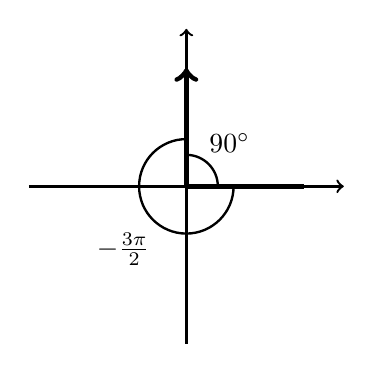
\begin{tikzpicture}
	\draw[line width=0.03cm,->] (-2,0) -- (2,0);				% x-axis
	\draw[line width=0.03cm,->] (0,-2) -- (0,2);				% y-axis
	
	\draw[line width=0.07cm,->] (0,0) -- (0,1.5);			% Initial Side
	\draw[line width=0.07cm] (0,0) -- (1.5,0);				% Terminal Side
	
	\draw[line width=0.03cm] (0.4,0) arc (0:90:0.4); \node at (0.55,0.55) {$90^\circ$};	% 90 deg
	\draw[line width=0.03cm] (0.6,0) arc (0:-270:0.6); \node at (-0.8,-0.8) {$-\frac{3\pi}{2}$};	% -3pi/2 
	\end{tikzpicture}
	\]



\newpage



% 10/09
\checkin{10/09} The point $(-0.888,0.460)$ is on the unit circle. If $\theta$ is the angle this point makes with the origin and positive $x$-axis, then $\sin \theta= -0.888$ and $\cos \theta= 0.460$. \pspace

\sol The statement is \textit{false}. Recall the points on the unit circle are of the form $(\cos \theta, \sin \theta)$. But then if $(-0.888,0.460)$ is on the unit circle, then $\cos \theta= -0.888$ and $\sin \theta= 0.460$. The given values are reversed. We can also do this using a sketch via reference angles. 
	\[
	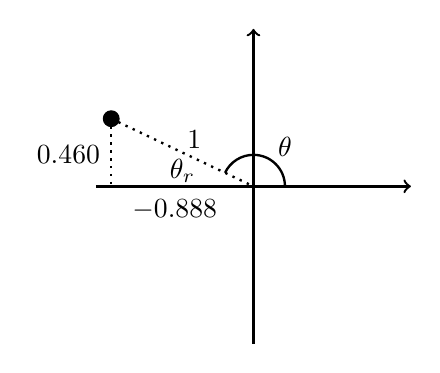
\begin{tikzpicture}
	\draw[line width=0.03cm,->] (-2,0) -- (2,0);				% x-axis
	\draw[line width=0.03cm,->] (0,-2) -- (0,2);				% y-axis
	
	\draw[fill=black] (-1.80613, 0.859016) circle (0.1);		% Point
	\draw[line width=0.03cm,dotted] (-1.80613, 0.859016) -- (-1.80613,0);	% Vertical Side
	\draw[line width=0.03cm,dotted] (-1.80613, 0.859016) -- (0,0);			% Horz. Side
	\draw[line width=0.03cm] (0.4,0) arc (0:154.564:0.4); \node at (0.4,0.5) {$\theta$};	% Arc

	\node at (-1,-0.3) {$-0.888$};	% Adj Label
	\node at (-2.35,0.4) {$0.460$};	% Opp Label
	\node at (-0.75,0.6) {$1$};		% Hypt. Label
	\node at (-0.9,0.2) {$\theta_r$};	% Reference Angle
	\end{tikzpicture}
	\]
But then $\sin \theta= \frac{\text{opp}}{\text{hyp}}= \frac{0.460}{1}= 0.460$ and $\cos \theta= \frac{\text{adj}}{\text{hyp}}= \frac{-0.888}{1}= -0.888$. \pvspace{1.3cm}



% 10/10
\checkin{10/10} $\cos(-120^\circ)= -\dfrac{\sqrt{3}}{2}$ \pspace

\sol The statement is \textit{false}. We plot the angle $-120^\circ$. We can see that the reference angle for $-120^\circ$ is $60^\circ$. We can see that $-120^\circ$ is in Quadrant~III, where $\cos \theta$ is negative. 
	\[
	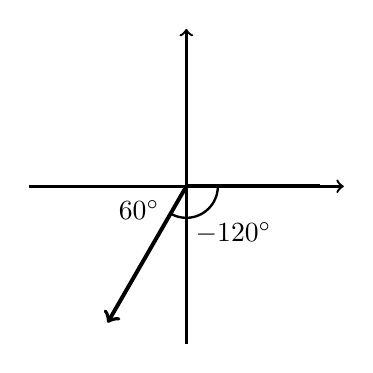
\begin{tikzpicture}
	\draw[line width=0.03cm,->] (-2,0) -- (2,0);				% x-axis
	\draw[line width=0.03cm,->] (0,-2) -- (0,2);				% y-axis
	
	\draw[fill=black,line width=0.05cm] (0,0) -- (1.7,0);		% Initial Side
	\draw[fill=black,->,line width=0.05cm] (0,0) -- (-1,-1.732);	% Terminal Side
	\draw[line width=0.03cm] (0.4,0) arc (0:-120:0.4);		% Angle Arc
	
	\node at (-0.6,-0.3) {$60^\circ$};	% 60 deg
	\node at (0.6,-0.6) {$-120^\circ$};	% -120 deg
	\end{tikzpicture}
	\]

Therefore, $\cos(-120^\circ)= - \cos(60^\circ)= -\frac{1}{2}$. 






























\end{document}